\documentclass[a4paper]{article}

\usepackage{amsmath}
\usepackage{amsthm}
\usepackage{amsfonts}
\usepackage[utf8]{inputenc}
\usepackage{csquotes}
\usepackage{listings}
\usepackage{graphicx}
\usepackage{ifthen}
\usepackage{xspace}
\usepackage{hyperref}
\usepackage{mathtools}
\usepackage{tikz}
\usepackage{caption}
\usepackage{subcaption}

\DeclarePairedDelimiter\ceil{\lceil}{\rceil}
\DeclarePairedDelimiter\floor{\lfloor}{\rfloor}

\newcommand{\pgap}{~\\\noindent}

\newcommand{\Fsh}{{F$\sharp$}\xspace}

\newcommand{\col}[2]{{\begin{pmatrix} #1 \\ #2 \end{pmatrix}}}
\newcommand{\mmod}{\text{ mod }}

\newtheorem{theorem}{Theorem}
\newtheorem{lemma}{Lemma}
\newtheorem{definition}{Definition}

\lstset{basicstyle=\small\ttfamily,frame=leftline,numbers=left,xleftmargin=0.7cm,basewidth=0.14cm}
\lstset{rangeprefix=(*, rangesuffix=*),includerangemarker=false}

\lstnewenvironment{Code}{}{}
\newcommand{\codeInput}[2][]{\ifthenelse{\equal{#1}{}}{\lstinputlisting[title=#2]{#2}}{\lstinputlisting[linerange=#1-end,title=#2\ -\ #1]{#2}}}
\newcommand{\code}{\lstinline}


\title{PoP 10g - Animals}
\author{Carl Dybdahl, Patrick Hartvigsen, Emil Søderblom}

\begin{document}

\maketitle

We have written a model of animals in \Fsh. Figure \ref{uml} shows the UML diagram we designed for this task. We have also written tests for our classes and documented their behavior.

\begin{figure}[!ht]
\centering
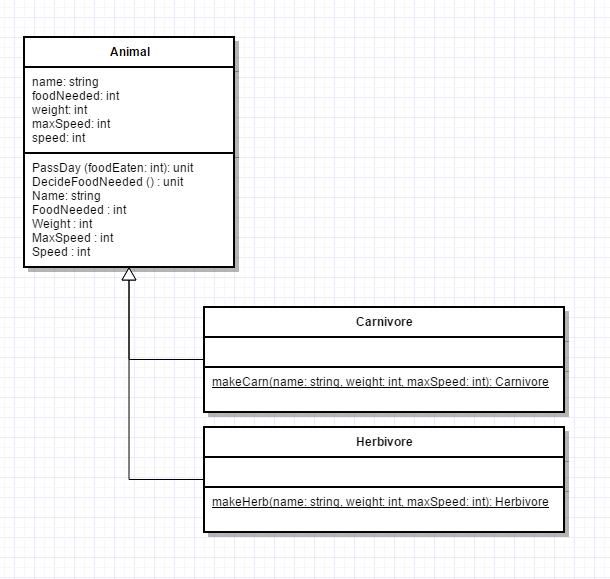
\includegraphics[width=0.5\textwidth]{animal_uml}
\caption{The UML diagram for the classes in this task.}
\label{uml}
\end{figure}

\section{Animal, Carnivore, Herbivore}

We have a base class \code|Animal| which implements most of the behavior of animals. It has five attributes, \code|Name|, \code|Weight|, \code|FoodNeeded|, \code|MaxSpeed| and \code|Speed|. In addition, it has two methods, \code|PassDay| and \code|DecideFoodNeeded|. We have written XML-comments to describe the exact details of these methods and attributes, but they can roughly be described as follows:

\begin{itemize}
\item \code|Name| and \code|Speed| do not directly affect anything else.
\item \code|PassDay| is given an amount of food eaten the current day and sets the \code|Speed| to a fraction of \code|MaxSpeed| based on how big a fraction of \code|FoodNeeded| is eaten.
\item \code|DecideFoodNeeded| sets the food needed to a fraction of the animal's \code|Weight|.
\end{itemize}

A \code|Carnivore| is an \code|Animal| that needs less food, whereas a \code|Herbivore| is an animal that needs more food. Semantically, \code|Carnivore|s represent carnivorous animals, whereas \code|Herbivore|s represent herbivorous animals.

We made the constructor of \code|Carnivore| and \code|Herbivore| private so we could make sure \code|DecideFoodNeeded| was called on every animal as soon as it is constructed. To create an instance of these classes, one must use the static members \code|makeCarn| and \code|makeHerb|.

\section{Race}

We have written the code to do a race between \code|cheetah|, a \code|Carnivore| weighing \(50\) kg and having a max speed of \(114\) km/hour; \code|antelope|, a \code|Herbivore| weighing \(50\) kg and having a max speed of \(95\) km/hour; and \code|wildebeest|, a \code|Herbivore| weighing \(200\) kg  and having a max speed of \(80\) km/hour.

The winner is declared to be the one who is the wins the most time in a test of three races on separate days, where each day the animals eat a random fraction of their \code|FoodNeeded|. If there is a draw, the race is retried.

\section{Documentation}

The code was documented according to the standard. In order to keep the documentation comments from cluttering up the code, we placed the documentation in the signature file \code|10g.fsi|.

\section{Tests}

We have tested all the methods and have gotten positive test results.

\end{document}